% ============================================================
% Figure 6: SNN vs KNN Graph Construction
% ============================================================
\documentclass[border=5pt]{standalone}
\usepackage[T1]{fontenc}
\usepackage{tikz}
\usetikzlibrary{arrows.meta, positioning, calc}

\definecolor{cb1}{RGB}{0,101,189}
\definecolor{cb2}{RGB}{204,51,51}
\definecolor{cb3}{RGB}{0,128,0}
\definecolor{cb5}{RGB}{117,112,179}

\begin{document}
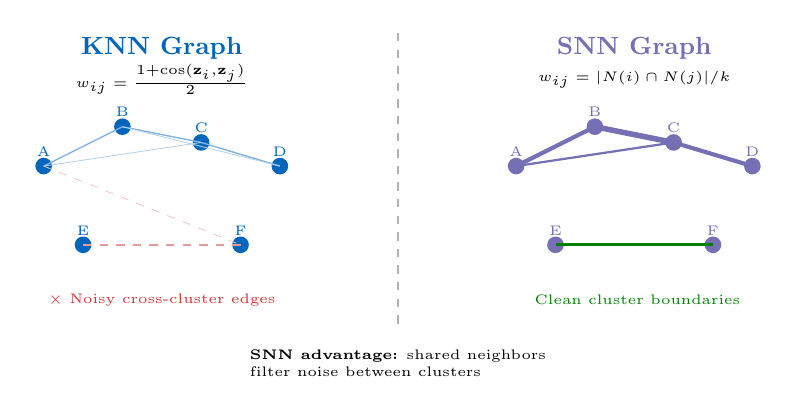
\begin{tikzpicture}[font=\scriptsize]

% ── KNN (left) ──
\node[font=\small\bfseries, cb1] at (2.5, 4) {KNN Graph};
\node[font=\tiny\itshape] at (2.5, 3.6) {$w_{ij} = \frac{1 + \cos(\mathbf{z}_i, \mathbf{z}_j)}{2}$};

% Points
\foreach \x/\y/\n in {1/2.5/A, 2/3/B, 3/2.8/C, 4/2.5/D, 1.5/1.5/E, 3.5/1.5/F} {
    \fill[cb1] (\x,\y) circle (3pt) node[above, font=\tiny] {\n};
}
% Edges (distance-based)
\draw[cb1!50, line width=0.5pt] (1,2.5) -- (2,3);
\draw[cb1!50, line width=0.5pt] (2,3) -- (3,2.8);
\draw[cb1!50, line width=0.5pt] (3,2.8) -- (4,2.5);
\draw[cb1!30, line width=0.3pt] (1,2.5) -- (3,2.8);
\draw[cb1!30, line width=0.3pt] (2,3) -- (4,2.5);
\draw[cb2!50, line width=0.5pt, dashed] (1.5,1.5) -- (3.5,1.5);
\draw[cb2!30, line width=0.3pt, dashed] (1,2.5) -- (3.5,1.5);

\node[font=\tiny, cb2] at (2.5, 0.8) {$\times$ Noisy cross-cluster edges};

% ── SNN (right) ──
\node[font=\small\bfseries, cb5] at (8.5, 4) {SNN Graph};
\node[font=\tiny\itshape] at (8.5, 3.6) {$w_{ij} = |N(i) \cap N(j)| / k$};

% Points
\foreach \x/\y/\n in {7/2.5/A, 8/3/B, 9/2.8/C, 10/2.5/D, 7.5/1.5/E, 9.5/1.5/F} {
    \fill[cb5] (\x,\y) circle (3pt) node[above, font=\tiny] {\n};
}
% Edges (shared-neighbor-based — thicker = more shared)
\draw[cb5, line width=1.5pt] (7,2.5) -- (8,3);
\draw[cb5, line width=2pt] (8,3) -- (9,2.8);
\draw[cb5, line width=1.5pt] (9,2.8) -- (10,2.5);
\draw[cb5, line width=0.8pt] (7,2.5) -- (9,2.8);

\draw[cb3, line width=1pt] (7.5,1.5) -- (9.5,1.5);
% No cross-cluster edges!

\node[font=\tiny, cb3] at (8.5, 0.8) {$\checkmark$ Clean cluster boundaries};

% Separator
\draw[black!30, dashed] (5.5, 0.5) -- (5.5, 4.2);

% Legend
\node[font=\tiny, align=left] at (5.5, 0) {
    \textbf{SNN advantage:} shared neighbors\\
    filter noise between clusters
};

\end{tikzpicture}
\end{document}
